% One-Page Pitch -- ISMC 2026, Track 2 "AI for MEMS"
%
% Build:  tectonic 01_one_page_pitch.tex
%
% HARD CONSTRAINT: one page. The budget is ~620 words of body text alongside
% the full-width capability strip. 9 pt, 0.5 in margins. Check the page count
% after every edit -- there is no slack.
%
% The four section names are taken from the call ("Problem statement, the AI
% approach, novelty, and impact on MEMS") so a reviewer working from the
% checklist can tick each one off the headings.
%
% Deliberately NOT here: the absolute-voltage / anchor-compliance caveat. The
% headline is a RELATIVE claim (22.86 -> 13.60 V within one process), which is
% exactly what the validation supports, so nothing here overstates. The full
% treatment is in the technical report's Conclusion.
\documentclass[9pt,twocolumn]{extarticle}
\usepackage[letterpaper,margin=0.5in]{geometry}
\usepackage{graphicx,amsmath,amssymb,booktabs,microtype}
\usepackage[T1]{fontenc}
\usepackage{titlesec}
\usepackage{xcolor}

\graphicspath{{../figures/}}

% Body text is plain black. Coloured headings read as a slide template rather
% than a technical document; the only colour on the page is inside the figures,
% where it carries data.
\titleformat{\section}{\normalfont\large\bfseries}{}{0pt}{}
\titlespacing*{\section}{0pt}{5pt}{1pt}
\setlength{\parskip}{2.5pt}
\setlength{\parindent}{0pt}
\setlength{\columnsep}{16pt}
\pagestyle{empty}

\begin{document}

\twocolumn[{%
\begin{center}
{\LARGE\bfseries Cutting MEMS Drive Voltage by 41\%
by Differentiating Through Pull-In\par}
\vspace{3pt}
{\small Tushar Dudeja, \emph{Student Member, IEEE}, and Nawaz Shafi,
\emph{Member, IEEE}\par}
\vspace{1pt}
{\small Vellore Institute of Technology, India\par}
\vspace{6pt}
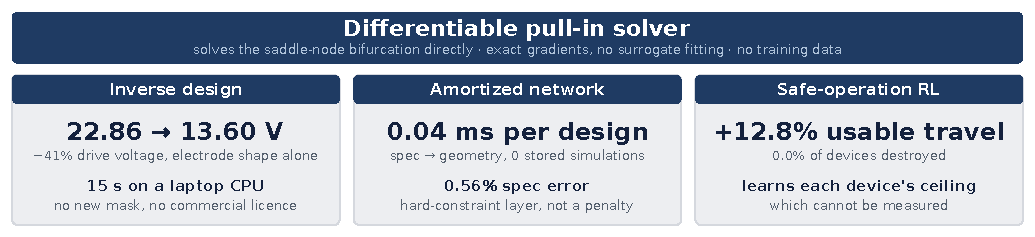
\includegraphics[width=0.95\textwidth]{Fig0b_pitch_strip.pdf}
\vspace{7pt}
\end{center}
}]

\section{Problem statement}

Electrostatic actuation drives most commercial MEMS: micromirror arrays, RF
switches, tunable capacitors and optical attenuators. Two limits bound all of
them, and both originate in pull-in.

Drive voltage is the first. Holding a useful deflection safely takes tens of
volts, well above any logic supply, so the die carries a charge pump that costs
area and quiescent power. Travel is the second: stable motion stops at a third
of the gap, at a threshold that moves with film thickness, residual stress and
etch bias. That threshold cannot be located without crossing it, and crossing
it destroys the device, so the drive schedule is set for the worst die on the
wafer and every good die is under-driven.

Designers meet this with FEM sweeps over hand-picked geometry families, in
tools that cost a licence and return a number with no derivative. Current AI
practice inherits the handicap: the standard pipeline fits a surrogate to
\textbf{48{,}000} simulations, then optimises through its approximation error.

\section{The AI approach, and its novelty}

We make the physics differentiable, including the instability itself.

Pull-in is a saddle-node bifurcation. At the fold the tangent stiffness is
singular, so a differentiated forward solve fails at precisely the point of
interest, which is one reason the problem is usually approached with
surrogates. Rather than approaching the fold, we solve for it: adding a
null-vector condition and a normalisation to the equilibrium residual gives
\begin{equation*}
R(Y,\Lambda)=0,\quad J(Y,\Lambda)\,v=0,\quad \|v\|=1,
\end{equation*}
which turns the bifurcation into an ordinary root of a regular system. Newton
lands on it directly, and the implicit function theorem then returns the
\textbf{exact} derivative of pull-in voltage with respect to every point of the
electrode gap, in one reverse pass.

\textbf{To our knowledge, no existing differentiable solver targets the
electrostatic pull-in bifurcation.} JAX-FEM, JAX-MPM and JaxSSO return
gradients through finite-element, meshfree and structural problems, but none
differentiates a fold point. Because the gradient comes from the physics rather
than from fitted data, \textbf{none of the three capabilities above requires a
training set}.

\section{Impact on MEMS}

\textbf{Drive voltage falls 22.86\,V $\rightarrow$ 13.60\,V, a 41\% reduction},
on the same beam meeting the same 2\,\textmu m travel specification. The
reduction comes entirely from reshaping the electrode gap, so it requires no
new material, no additional process step and no additional mask.

The optimiser reaches it in \textbf{15 seconds on a laptop CPU} without a
commercial licence, starting from a uniform gap and given no information about
any prior design family. Once trained, the network emits a geometry in
\textbf{0.04\,ms}, against the 48{,}000 stored simulations the standard
pipeline requires beforehand.

For device operation, a policy observing only a device's own tilt response
infers the unmeasurable ceiling and recovers \textbf{12.8\% more usable travel
with 0.0\% of devices destroyed}, over 1{,}536 held-out test episodes.

The same machinery addresses a question left open in the literature. Haluzan
\emph{et al.} (2010) conjectured that gains beyond simple gap shapes ``are
believed to be minimal'' but had no means to test it. Free-form optimisation
quantifies what remains: \textbf{0.14\%} for the cantilever and
\textbf{1.45\%} for the fixed--fixed beam.

\section{Evidence}

The solver is validated against \textbf{eight independent sources published
between 1967 and 2025}, of which two are the most discriminating. The exact
gradient reproduces an analytic cube-scaling law to \textbf{0.00\%}; this tests
the differentiation itself rather than the forward solve, and would expose a
plausible but incorrect adjoint. Second, the optimal gap exponent
\emph{reverses} between geometries, approximately $4/3$ for a cantilever
against exactly $1$ for a fixed--fixed beam, and both are reproduced. Opposite
trends in two geometries are not obtainable by fitting. Three of three
instability mechanisms reported by Seeger and Boser are also predicted
correctly.

The full implementation is released: solver, validation suite, RL environment,
the MLP and Fourier-neural-operator baselines used for comparison, and a
ninety-second demonstration notebook. No commercial licence is required at any
stage, so the results reported here are reproducible on a laptop CPU.

\vspace{4pt}
% Placed inline rather than as a float: it is the last element on the page and
% a [t] float would jump to the top of column 1, above the title block.
\begin{center}
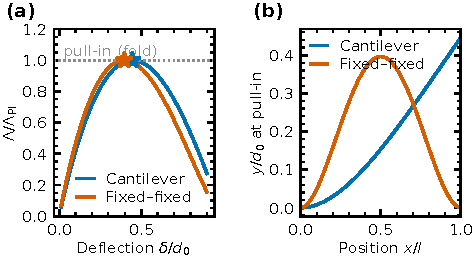
\includegraphics[width=0.94\columnwidth]{Fig3_fold_structure.pdf}
\vspace{-2pt}

{\footnotesize\textbf{The object we differentiate.} The load maximum
\emph{is} pull-in, the saddle-node our solver targets directly.\par}
\end{center}

\end{document}
